According to A. E. Vinogradov's research paper, it was found that higher GC counts did not correlate with higher thermostability, in fact higher counts of GC had lower levels of thermostability.

With increased elevation of GC percentages it was seen that bendability also increased, which would suggest that places in genome with higher counts of GC would result in increased expression.

In the Figure 1. you can see the average percentages of CLIB215 yeast species. We can clearly see that the percentages of CG bases are really similar, around 38 percent. The key difference is that the second image of the GC count have much more outliers than the first one.
\begin{figure}[htbp]
  \centering
  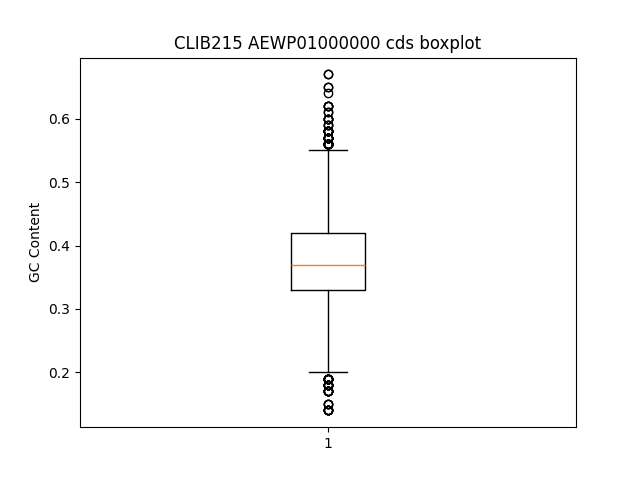
\includegraphics[width=0.45\textwidth]{images/CLIB215_AEWP01000000_cds_boxplot.png}
  \hfill
  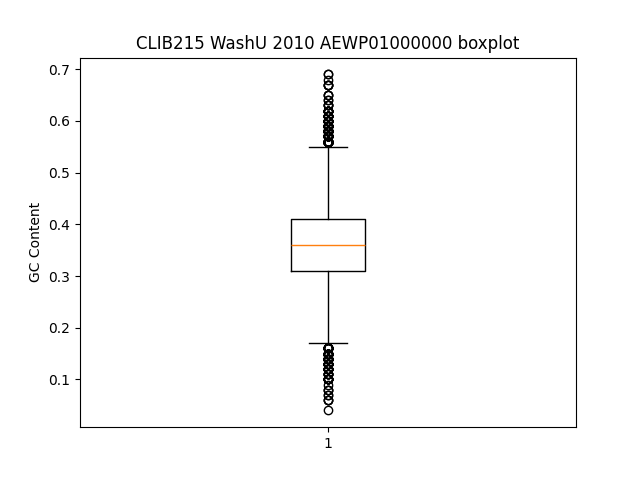
\includegraphics[width=0.45\textwidth]{images/CLIB215_WashU_2010_AEWP01000000_boxplot.png}
  \caption{GC counts of CLIB215 yeast species (percentage)}
  \label{fig:combined-images}
\end{figure}

Figure 2. provides us with a similar result as the first one, with slightly higher percentages, around 39 percent in the first image and 35 percent in the second one. Second one also having more outliers.
\begin{figure}[htbp]
  \centering
  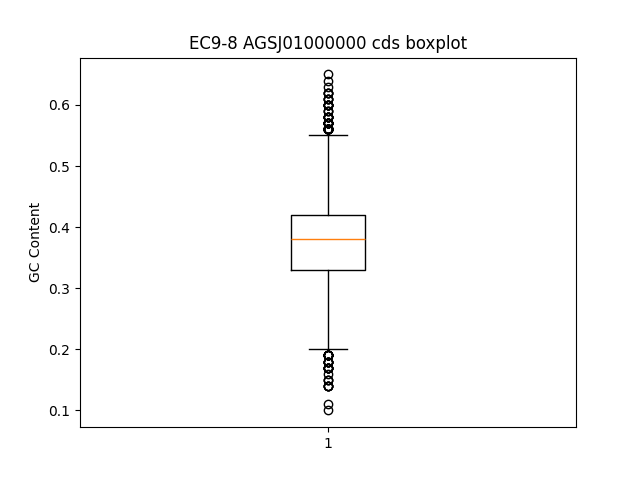
\includegraphics[width=0.45\textwidth]{images/EC9-8_AGSJ01000000_cds_boxplot.png}
  \hfill
  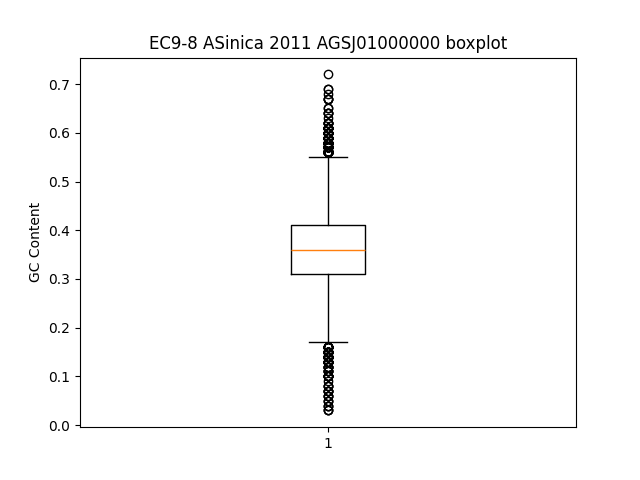
\includegraphics[width=0.45\textwidth]{images/EC9-8_ASinica_2011_AGSJ01000000_boxplot.png}
  \caption{GC counts of EC9-8 yeast species (percentage)}
  \label{fig:combined-images}
\end{figure}



